\documentclass{beamer}

\usepackage{minted}
\usepackage{tikz}
\usepackage{todonotes}

\setminted{frame=single}

\usetheme{codecentric}
\author{Markus Hauck}
\institute{codecentric AG}

\title{Functional Web Services}

\hypersetup{colorlinks,linkcolor=beamer@ccblue}

\begin{document}
{
  \usebackgroundtemplate{\includegraphics[width=\paperwidth,height=\paperheight]{background.png}}
  \begin{frame}[plain,noframenumbering]
    \titlepage{}
  \end{frame}
}

\section{Intro}

\begin{frame}
  \begin{center}
    \huge
    What are we gonna do tonight?
  \end{center}
\end{frame}

\begin{frame}
  \begin{center}
    
\includegraphics[width=0.7\paperwidth]{pics/pinkybrain.jpg}
  \end{center}
\end{frame}

\begin{frame}
  \frametitle{What are we going to do tonight}
  \begin{minipage}{0.2\linewidth}
    
\includegraphics[width=0.19\linewidth]{pics/scalpel.png}
  \end{minipage}
  \begin{minipage}{0.7\linewidth}
    \begin{itemize}
    \item write a small web service
    \item with http4s
    \item using an embedded DSL
    \item emphasize functional style
    \end{itemize}
  \end{minipage}
  \vfill
  \begin{center}
    \url{https://github.com/markus1189/runnersparadise}
  \end{center}
\end{frame}

\begin{frame}
  \frametitle{Embedded DSLs}
  \begin{itemize}
  \item embedded in general purpose language
  \item functional: separate \texttt{description} of program from
    \texttt{execution}
  \item initial encoding: \texttt{Free Monads}
  \item final encoding: \texttt{typeclasses + instances}
  \item also: deep vs shallow embedding
  \end{itemize}
\end{frame}

\section{A First DSL}

\begin{frame}
  \frametitle{A First DSL}
  \begin{center}
    
\includegraphics[width=2cm]{pics/owl.png}
  \end{center}
  \begin{itemize}
  \item let's start with our first DSL
  \item arithmetic operations: \texttt{+} and \texttt{-} (negation)
  \item how would you do this in an initial encoding?
  \end{itemize}
\end{frame}

\begin{frame}[fragile,fragile]
  \frametitle{Initial Encoding}
\begin{minted}{scala}
sealed trait Exp
case class Lit(x: Int)           extends Exp
case class Neg(e: Exp)           extends Exp
case class Add(e1: Exp, e2: Exp) extends Exp
\end{minted}
  \begin{itemize}
  \item writing a program
  \end{itemize}
\begin{minted}{scala}
//(8 + -(1 + 2))
Add(Lit(8),
    Neg(Add(Lit(1),
            Lit(2))))
\end{minted}
\end{frame}

\begin{frame}
  \frametitle{Properties of the Initial Encoding}
  \begin{itemize}
  \item nice to have ADT with possible cases
  \item flexible interpretation, evaluate, pretty print, \dots{}
  \item bad: extending with e.g.\ multiplication is not independent
  \item let's try something different: \texttt{final encoding}
  \end{itemize}
\end{frame}

\begin{frame}
  \begin{center}
    \Huge Live Coding: Our first DSL
  \end{center}
  \begin{center}
    
\includegraphics[width=0.7\textwidth]{pics/penguins.jpg}
  \end{center}
\end{frame}

\begin{frame}[fragile]
  \setminted{frame=none}
  \frametitle{Review: Final Encoding}
  \begin{minipage}[frame=none]{0.45\linewidth}
\begin{minted}{scala}
sealed trait Exp[A] {
  def lit(x:Int): A
  def neg(e:A): A
  def add(e1 A, e2:A): A
}
\end{minted}
  \end{minipage}
  \begin{minipage}[frame=none]{0.45\linewidth}
\begin{minted}{scala}
new Exp[Int] {
  def lit(x:Int) = x
  def neg(e: Int) -e
  def add(e1:Int,e2:Int) =
    e1 + e2
  }
\end{minted}
  \end{minipage}
  \begin{itemize}
  \item define typeclass for syntax
  \item define instance for semantics
  \item typeclass also called \texttt{Symantics}
  \item languages are independent, expressed via constraints on types
  \end{itemize}
\end{frame}

\section{Web Services with Http4s}

\begin{frame}
  \begin{center}
    \Huge Web Services with Http4s
  \end{center}
\end{frame}

\begin{frame}{http4s}
  \begin{block}{What is \hyperlink{http://http4s.org/}{http4}}
    A typeful, purely functional, streaming library for HTTP
    clients and servers in Scala.
  \end{block}
  \begin{itemize}
  \item typeful \textemdash{} self-documentation and compile-time verification
  \item purely functional \textemdash{} promote composability and reasoning
  \item streaming \textemdash{} large payloads in constant space and websockets
  \end{itemize}
\end{frame}

\begin{frame}[fragile]
  \frametitle{Writing Web Services With Http4s}
  \begin{itemize}
  \item define \texttt{HttpService} using the built-in DSL
  \item \texttt{really} just \texttt{Request => Task[Response]}
  \item (\texttt{Task[A]} is a better \texttt{Future[A]})
  \item define routes via pattern matching:
  \end{itemize}
\begin{minted}{scala}
HttpService {
  case req @ GET -> Root / "hello" =>
    handleHelloWorld(req)
}
\end{minted}
\end{frame}

\section{Runner's Paradise DSL}

\begin{frame}
  \frametitle{Our Domain}
  \begin{center}
    \huge
    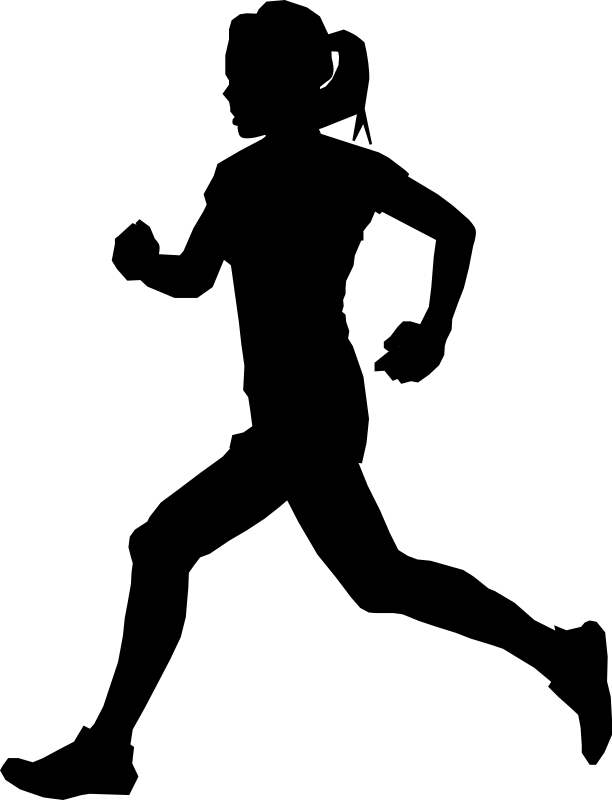
\includegraphics[width=2cm]{pics/runner.png}
    Runners
    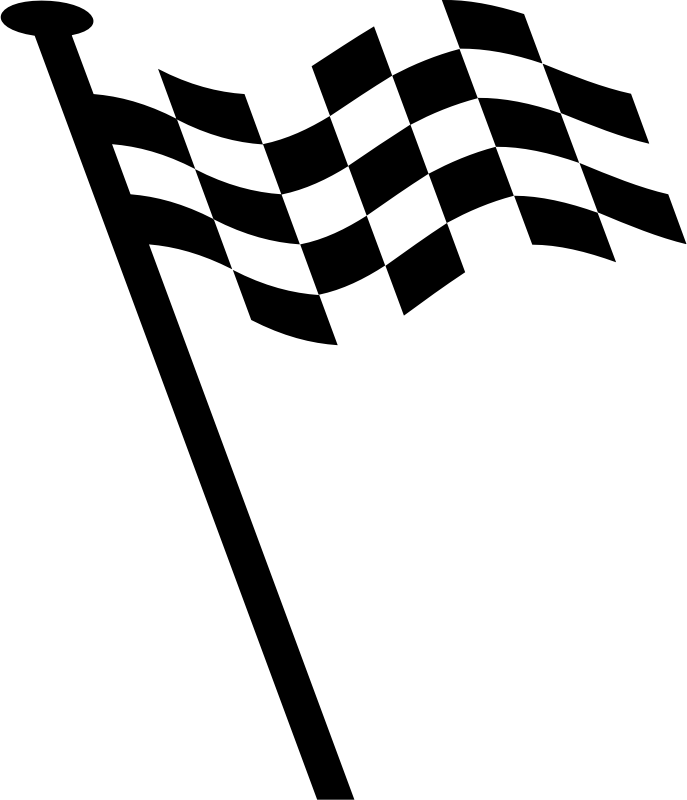
\includegraphics[width=2cm]{pics/race.png}
    Races
    
\includegraphics[width=2cm]{pics/registration.png}
    Registrations
  \end{center}
\end{frame}

\begin{frame}[fragile]
  \frametitle{Our API}
\begin{minted}{scala}
GET  "localhost/runner/<runner-id>"
GET  "localhost/race/<race-id>"
GET  "localhost/registration/<race-id>"
PUT  "localhost/registration"
POST "localhost/runner"
POST "localhost/race"
\end{minted}
\end{frame}

\begin{frame}[fragile]
  \frametitle{Our API}
\begin{minted}{scala}
case GET -> Root / "runner" / RunnerIdVar(rid)
case GET -> Root / "race" / RaceIdVar(rid)
case GET -> Root / "registration" / RaceIdVar(rid)
case req @ PUT -> Root / "registration"
case req @ POST -> Root / "runner"
case req @ POST -> Root / "race"
\end{minted}
\end{frame}

\begin{frame}[fragile]
  \frametitle{The Runners Paradise DSL}
\begin{minted}{scala}
trait RunnerAlg[F[_]] {
  def saveRunner(runner: Runner): F[Unit]
  def findRunner(id: RunnerId): F[Option[Runner]]
}
\end{minted}
  \begin{itemize}
  \item we use a \textit{higher-kinded} type \texttt{F}
  \item kind: \texttt{* -> *}, i.e.\ it needs another type of kind
    \texttt{*}
  \item results are wrapped in \texttt{F[\_]}
  \item \textit{instances choose the concrete F}
  \end{itemize}
\end{frame}

\begin{frame}[fragile]
  \frametitle{The Runners Paradise DSL}
\begin{minted}{scala}
trait RaceAlg[F[_]] {
  def saveRace(race: Race): F[Unit]
  def findRace(id: RaceId): F[Option[Race]]
}
\end{minted}
\begin{minted}{scala}
trait RegistrationAlg[F[_]] {
  def saveReg(reg: Registration): F[Unit]
  def findReg(id: RaceId): F[Option[Registration]]
}
\end{minted}
\end{frame}

\begin{frame}
  \frametitle{The Runners Pradise DSL: Registrations}
  \begin{itemize}
  \item allow registration of runners for races
  \item if:
    \begin{itemize}
    \item race exists
    \item runner exists
    \item race has free slots
    \end{itemize}
  \item reality: \texttt{Either[RegistrationError,Registration]}
  \end{itemize}
\end{frame}

\begin{frame}
  \frametitle{Fair Warning: Fancy Code Incoming}
  
\includegraphics[width=\textwidth]{pics/warning.png}
\end{frame}

\begin{frame}[fragile]
  \frametitle{The Runners Paradise DSL}
\begin{minted}[fontsize=\footnotesize]{scala}
def registerOpt[F[_]:Monad:RunnerAlg:RaceAlg:RegistrationAlg](
      runnerId: RunnerId,
      raceId: RaceId): F[Option[Registration]] = {

    val M = Monad[OptionT[F, ?]]

    for {
      runner <- OptionT(RunnerAlg().findRunner(runnerId))
      race   <- OptionT(RaceAlg().findRace(raceId))
      reg    <- OptionT(RegistrationAlg().findReg(raceId)).
                  orElse(M.point(Registration(race, Set())))
      newReg <- OptionT(reg.add(runner).pure[F])
      _      <- OptionT(RegistrationAlg().saveReg(newReg).
                  map(Option(_)))
    } yield newReg
  }.run
\end{minted}
\end{frame}

\begin{frame}[fragile]
  \frametitle{Registration Program}
\begin{minted}{scala}
def registerOpt[F[_]:             // still abstract
                Monad:            // flatMap
                RunnerAlg:        // runners
                RaceAlg:          // races
                RegistrationAlg]( // registrations
  runnerId: RunnerId,             // runner id
  raceId: RaceId                  // race id
): F[Option[Registration]]        // wrapped in F
\end{minted}
\end{frame}

\begin{frame}
  \frametitle{Getting More Concrete: Instances}
  \begin{itemize}
  \item to actually run programs, we need to have instances
  \item need to satisfy \texttt{all} constraints
  \item pure in-memory, cassandra, postgres, redis, \dots{}
  \end{itemize}
\end{frame}

\begin{frame}[fragile,fragile]
  \frametitle{Instances for our DSL}
\begin{minted}{scala}
class Cass[A](
  val value: ReaderT[Task, RunnersParadiseDb, A]
) extends AnyVal {
  def run: RunnersParadiseDb => Task[A] = value.run
}
\end{minted}
  \begin{itemize}
  \item \texttt{RunnersParadiseDb => Task[A]}
  \item given a connection to the DB, asynchronous results
  \end{itemize}
\end{frame}

\begin{frame}[fragile,fragile]
  \frametitle{Instances for our DSL}
\begin{minted}{scala}
class Cass[A](
  val value: ReaderT[Task, RunnersParadiseDb, A]
) extends AnyVal {
  def run: RunnersParadiseDb => Task[A] = value.run
}
\end{minted}
  \vfill
\begin{minted}{scala}
def saveRunner(runner: Runner): Cass[Unit] =
  new Cass(ReaderT(_.runners.save(runner).void))
\end{minted}
\end{frame}

\section{Final Encodings and http4s}

\begin{frame}[fragile]
  \frametitle{Putting It Together}
  \begin{itemize}
  \item remember signature of routes?
  \end{itemize}
\begin{minted}{scala}
Request => Task[Response]
\end{minted}
  \begin{itemize}
  \item at the end our program \textbf{has} to produce a \texttt{Task}
  \item but we don't want to be limited by this
  \end{itemize}
\end{frame}

\begin{frame}
  \frametitle{Let's Have A Look}
  \begin{center}
    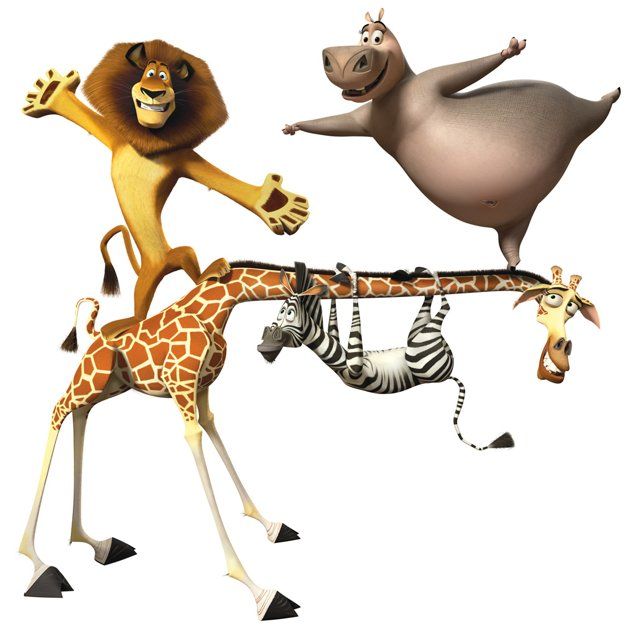
\includegraphics[width=0.5\textwidth]{pics/review.jpg}
  \end{center}
\end{frame}

\section{Testing}

\begin{frame}[fragile]
  \frametitle{Typeclasses Need Laws}
  \begin{itemize}
  \item<1-> typeclasses should \textit{always} come with laws
  \item<1-> what about \texttt{RunnerAlg}?
  \end{itemize}
\begin{minted}{scala}
trait RunnerAlg[F[_]] {
  def saveRunner(runner: Runner): F[Unit]
  def findRunner(id: RunnerId): F[Option[Runner]]
  def listRunner: F[Vector[Runner]]
}
\end{minted}
  \begin{itemize}
  \item<2-> \texttt{saveRunner *> saveRunner}
  \item<2-> \texttt{findRunner *> findRunner}
  \item<2-> \texttt{saveRunner *> findRunner}
  \item<2-> \texttt{saveRunner *> listRunners}
  \end{itemize}
\end{frame}

\begin{frame}[fragile]
  \frametitle{ScalaCheck}
  \begin{itemize}
  \item ScalaCheck is perfect for checking our laws
  \item defined in terms of \texttt{RunnerAlg[F[\_]]}
  \end{itemize}

\begin{minted}{scala}
forAll { (runner: Runner) =>
  run {
    RunnerAlg().saveRunner(runner) *>
      RunnerAlg().findRunner(runner.id)
  }.value should ===(runner)
}
\end{minted}
  \begin{itemize}
  \item instantiate this test for our instances
  \item pure in memory, cassandra, postgres, \dots{}
  \end{itemize}
\end{frame}

\begin{frame}
  \frametitle{Review of Final Encodings}
  \begin{itemize}
  \item initial encoding is not always the best
  \item final encoding is easier to extend
  \item btw: nice way to solve expression problem (exercise)
  \item you can \textit{always} convert between initial and final
  \end{itemize}
\end{frame}

\begin{frame}
  \frametitle{Further References}
  \begin{itemize}
  \item Oleg Kiselyov: Lecture notes on
    \href{http://okmij.org/ftp/tagless-final/course/lecture.pdf}{Typed
      Tagless Final Interpreters}
  \item Runner's Paradise Code: \url{https://github.com/markus1189/runnersparadise}
  \end{itemize}
\end{frame}

\begin{frame}
  \frametitle{Questions}
  \begin{center}
    
\includegraphics[width=0.5\textwidth]{pics/questions.png}
  \end{center}
\end{frame}

\end{document}
